\chapter{Game and AI Framework Implementation}

The framework in Durak is tailored to support the implementation and evaluation of artificial intelligence algorithms within the game environment. The main objective of the it is to provide a framework for the development and testing of AI agents, aiming to evaluate their performance within the game. This chapter presents a high-level overview of the game and AI framework, including its capabilities for supporting the development and evaluation of AI for Durak. 

A more in-depth analysis of the implementation and functionality of the game model can be found in section \ref{devdoc} of the developer documentation, as well as in the user documentation provided in section \ref{userdoc}. These sections provide comprehensive information on the design and implementation of the game model, as well as its capabilities and usage for both developers and end users.

\section{OS support}

The game framework for Durak was tested on both Windows 10 and Linux operating systems to confirm compatibility and functionality. While this list is not exhaustive, and the framework may potentially run on other operating systems, these are the only ones that were formally tested. It is possible that the framework will operate correctly on other platforms, but this has not been verified.

\section{Design}

The Durak AI framework includes a game model, AI agents, and a Command-Line Interface (CLI) that are implemented using the C\# programming language and targeted for the .NET Core 6 platform.

C\# was selected as the programming language for the implementation of aforementioned projects in Durak due to its suitability for writing back-end systems. The language offers a range of reliable libraries and benefits from a highly optimized Just-In-Time (JIT) compiler, resulting in enhanced speed. These attributes made C\# an ideal choice for this development.

In order to run and test the program, the project has to be cloned from the repository and opened with an Integrated Development Environment (IDE) of user's choice. From the root directory of the project, the user can utilize the command line to enter the command 
\begin{verbatim}
dotnet run --project CLI
\end{verbatim}
, which will launch the Command-Line Interface (CLI) and provide guidance on how to proceed with experimentation. The CLI will provide further instructions on how to use and test the program (for additional information, please refer to Section \ref{CLI}.).

\subsection{Project Structure}
The game Durak is organized within a solution file, with the file extension ``.sln'', which is a type of file used to manage projects in Visual Studio. This solution includes three individual projects: 

\begin{itemize}

\item Model - A C\# library project contains the game logic for Durak.

\item Agent - A C\# library contains all of the implemented AI agents.

\item CLI - A C\# Command-Line Interface (CLI) project includes parameters for modifying the game model and agents settings in order to perform experiments.

The aforementioned mentioned components will be further discussed in the following subsections.

\end{itemize}

\subsection{Game Model}

The game model, which represents the current state of the game, is implemented using object-oriented programming principles. As it was mentioned before, the game logic for Durak is contained within the \textbf{Model} C\# library, which serves as a modular and reusable unit. It includes class objects, such as Player, Card, and Deck, as well as all of the other main components that make up the game each of which is equipped with the necessary methods to support the game's functionality. These objects and their methods are designed to reflect the key components and features described in the game description.

Before delving into the description of the game state and components of Durak, it is useful to first consider the relationship of all of the objects in the model to that state. A class diagram illustrating the relationships between the objects in the model can be found in Figure \ref{fig:modelUML}.


\begin{figure}[h]
    \centering
    \captionsetup{justification=centering}
    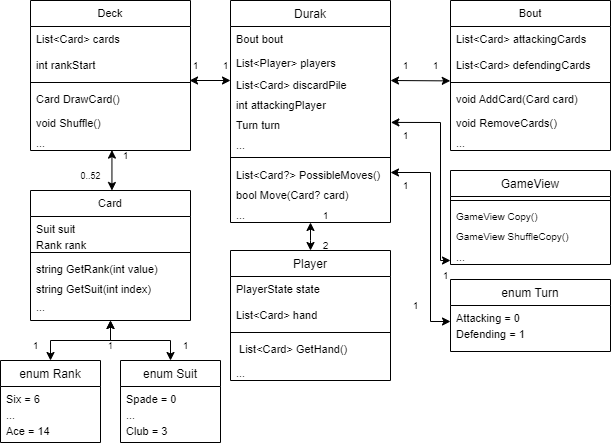
\includegraphics[width=0.70\textwidth]{../img/modelUML.png}
    \caption{A UML diagram showing the relationship between the objects within the Model library.}
    \label{fig:modelUML}
\end{figure}

\subsection{CLI}
\label{CLI}

\subsection{AI Agents}

\section{Interface}
